% File: project_notebook.tex
% Description: TeX file to generate Project Notebook (template)
% Author: George Hadley
% Website: http://nbitwonder.com
% Notes:
% 1) This document is written using the LaTeX typesetting language. For more information on
%	LaTeX, consult http://en.wikibooks.org/wiki/LaTeX/
% 2) This document needs to be compiled using pdfLaTeX. It is not supported with pdfTeX
%	at the present time
% 3) This document utilizes the \nbwheader command created in doc_header.tex. By default,
%	this file is located at:
%	/path-to-documentation-templates/lbr/doc_header.tex
% 4) This document utilizes commands and environments created in projnb_lbr.tex. By default,
%	this file is located at:
%	/path-to-documentation-templates/lbr/projnb_lbr.tex
% Version: 0.1
% Last Modified: 1-04-2010
\documentclass[12pt,letterpaper,onecolumn]{article}
\usepackage{graphicx}
\usepackage{float}
\usepackage{subfig}
\usepackage{tikz}
\usepackage{fancyhdr}
%\usepackage{kpfonts}  %Uncomment if kpfonts is installed and you want to use a non-default font
\usepackage{verbatim}
\usepackage{fullpage}
\usepackage{hyperref}
\usepackage{parskip}

%Path to global documentation library functions
%Modify this to /path-to-documentation-templates/lbr
\newcommand{\globallbr}{../lbr}

%Page layout settings
\setlength{\voffset}{-10pt}
\setlength{\headsep}{20pt}
\setlength{\headheight}{15pt}
\setlength{\topmargin}{-20pt}

\begin{comment}
  Hyperref settings: settings for the hyperref hyperlink package.
  For a more detailed listing of available settings, consult 
  	http://en.wikibooks.org/wiki/LaTeX/Hyperlinks#Customization

  IMPORTANT: For your document, modify the pdftitle, pdfauthor, pdfsubject,
	and pdfkeywords options to tailor to your document
\end{comment}
\hypersetup{
	bookmarks=true, 					%Enable pdf bookmarks
	pdfborder={0,0,0},					%Disable borders around links
	pdftitle={Class-D Amp Design Notebook)},		%Name of PDF document
	pdfauthor={Ben Laskowski},				%Author of PDF document
	pdfsubject={Embedded Electronics},		%Subject of PDF document
	pdfkeywords={diy,electronics,nbitwonder},	%Keywords for PDF document
	colorlinks={true},					%Enable colored links
	linkcolor=red,						%Internal link color
	citecolor=green,						%Citation link color
	filecolor=blue,						%File link color
	urlcolor=blue						%URL link color
}
% File: doc_header.tex
% Description: TeX command used to develop custom documentation header used in Open
%	 Documentation System
% Author: George Hadley
% Website: http://nbitwonder.com
% Notes: 
% 1) Derived from LaTeX example 'TeXblog: Fancy chapter headings with TikZ' found at
%	http://texblog.net/latex-archive/layout/fancy-chapter-tikz/
% 2) For additional help with the LaTeX package, consult the WikiBook found at
%	http://en.wikibooks.org/wiki/LaTeX
% 3) This file needs to be compiled with pdfLaTeX (does not appear to be compatible with
%	pdfTeX at the present time)
% Version: 0.1
% Last Modified: 12-28-2010

%Variable Declarations (modify these to tweak the header on your document)
\newcommand{\headery}{-3cm}					%y-offset of header (bottom left corner of header)
\newcommand{\headercolor}{black}				%Background color of header
\newcommand{\headerxstart}{.1\paperwidth}			%Starting x-coordinate for header box
\newcommand{\headerystart}{0cm}				%Starting y-coordinate for header box
\newcommand{\headerxend}{.9\paperwidth}			%Ending x-coordinate for header box
\newcommand{\headeryend}{2cm}				%Ending y-coordinate for header box
\newcommand{\logoxstart}{.1\paperwidth}			%Starting x-coordinate for logo
\newcommand{\logoystart}{1cm}					%Starting y-coordinate for logo
\newcommand{\logolink}{http://nbitwonder.com}		%URL for website, etc.
\newcommand{\logoheight}{40pt}					%Height of logo image
\newcommand{\logoloc}{../lbr/img/NBitWonderLogo_wTm.png}	%Path to logo image
\newcommand{\docboxxstart}{.5\paperwidth}		%Starting x-coordinate of documentation box
\newcommand{\docboxystart}{1cm}				%Starting y-coordinate of documentation box
\newcommand{\docboxwidth}{.38\paperwidth}		%Width of documentation box
\newcommand{\docboxtextcolor}{green}			%Text color in documentation box

% Command: \nbwheader
% Description: Creates a documentation header for use in the Open Documentation System templates
% Usage: \nbwheader{DocumentName}{ProjectName}{ProjectVersion} where
%	DocumentName is the name of the document (e.g. Project Notebook, User Manual, Bug Tracker, etc.
%	ProjectName is the name of the project the documentation is about
%	ProjectVersion is the current version of the project
\newcommand{\nbwheader}[3]
{
    \begin{tikzpicture}[remember picture,overlay]
    \node[yshift=\headery] at (current page.north west)
    {
        \begin{tikzpicture}[remember picture, overlay]
        \draw[fill=\headercolor] (\headerxstart,\headerystart) rectangle
            (\headerxend,\headeryend);
        \node[anchor=west,xshift=\logoxstart,yshift=\logoystart,rectangle]
        {\href{\logolink}{\includegraphics[height=\logoheight]{\logoloc}}};
        \node[anchor=west,xshift =\docboxxstart,yshift=\docboxystart,rectangle]
        {
            \begin{minipage}{\docboxwidth}
	   \begin{flushright}
	   \normalsize\textcolor{\docboxtextcolor}{\textsc{
	   \linespread{2}
	   #1 \\
	   Project: #2 \\
	   Version: #3 \\
            }}
	   \end{flushright}
            \end{minipage}};
        \end{tikzpicture}
        };
    \end{tikzpicture}
}

% File: aliases.tex
% Description: TeX library aliases used in open documentation templates
% Author: George Hadley
% Website: http://nbitwonder.com
% Notes: 
%	1) For additional help with the LaTeX package, consult the WikiBook found at
%		http://en.wikibooks.org/wiki/LaTeX
%	2) This file needs to be compiled with pdfLaTeX (does not appear to be compatible with
%		pdfTeX at the present time)
% Version: 0.1
% Last Modified: 1-04-2010
\newcommand{\ohm}{$\Omega$}
\newcommand{\uF}{$\mu$F}
% File: project_notebook_lbr.tex
% Description: TeX commands used for the project notebook in the Open 
%	Documentation System
% Author: George Hadley
% Website: http://nbitwonder.com
% Notes:
% 1) This document was written using the LaTeX typesetting language. For more help
%	with the LaTeX typesetting language, consult: http://en.wikibooks.org/wiki/LaTeX/
% 2) This file needs to be compiled with pdfLaTeX (does not appear to be compatible with
%	pdfTeX at the present time
% Version: 0.0
% Last Modified: 12-28-2010

% Variable Declarations: \projnbtagline command

% Command: \projnbtagline
% Description: Creates a tagline for use in the Project Notebook entries
% Usage: \projnbtagline{Entry#}{Date}{Version}{Title} where
% 	Entry# is the number of the current entry
%	Date is the date of the current entry
%	Version is the version number of the current entry (major and minor version)
%	Title is a short, descriptive title of the project entry
\newcommand{\projnbtagline}[4]
{
\textbf{Entry:} #1 \textbf{Date:} #2 \textbf{Version:} #3 \textbf{Title:} #4
\hfill
}

%Variable declarations: \nbentry environment

% Environment: nbentry
% Description: Environment defined for project notebook entries
% Usage: \begin{nbentry}{Entry#}{Date}{Version}{Title} where
% 	Entry# is the number of the current entry
%	Date is the date of the current entry
%	Version is the version number of the current entry (major and minor version)
%	Title is a short, descriptive title of the project entry

\newenvironment{nbentry}[4]
{\noindent\framebox[\textwidth]{\projnbtagline{#1}{#2}{#3}{#4}}\hfill\newline}
{\hfill\newline}


%Modify these to reflect your documentation
\newcommand{\documentationtype}{Project Notebook}
\newcommand{\projectname}{Class D Amplifier }
\newcommand{\projectversion}{1.0}

%Header/Footer Definitions
\pagestyle{fancy}
\lhead{ }
\chead{ }
\rhead{\projectname  v\projectversion  \documentationtype}
\lfoot{\href{http://nbitwonder.com}{http://nbitwonder.com} }
\cfoot{\thepage}
\rfoot{\copyright 2011 NBitWonder}

\begin{document}
\thispagestyle{plain}
% Insert title page or header here
\nbwheader{\documentationtype}{\projectname}{\projectversion}
% Insert optional project index here
% For long projects, it is recommended that project entries be indexed
%	by entry, week, month, or year (or a combination of the above)

% Project Notebook entries
% Project Notebook entries should be enclosed in boxes and contain a tagline
%	detailing the entry number, date, revision (project minor version), and 
%	a short, descriptive title
\begin{nbentry}{001}{1/27/2011}{1.00}{Defining requirements}
After the overwhelming success of the Class-D audio amplifier, it was decided to pursue an impoved, less experimental version.  Some ideas for the revised circuit include using entirely surface mount parts (reduced size and potentially increased performance), a higher supply voltage (increased power output), and an output inductor with a lower series resistance.

Other ideas brought forward for consideration are the use of a different class, such as Class G, Class H, Class I, or Class T.  These ideas were rejected due to potential copyright/patent issues and complexity.
\end{nbentry}

\begin{nbentry}{002}{1/29/2011}{1.00}{Initial BOM}
This post is duplicated from the NBitWonder Forums.

After some research, I've arrived at a partial bill of materials.

\begin{itemize}
\item MOSFETs - DMN4009
\item Gate driver - IRS2004
\item Comparator - LM311
\item Integrating error amp - TL082
\end{itemize}

The amplifier will, like the prototype, be a self-oscillating type. My hope is that with proper construction techniques, the operating frequency will be quite high, ideally upwards of 500kHz. To that end, the output filter has been designed as a second-order Butterworth filter with a cutoff of 50kHz when operated with an 8-ohm speaker, a common value for home use. An inductor has been identified with a very low series resistance, which should help efficiency improve over the prototype.

The MOSFETs selected for use this time are cheaper than the IRL520Ns used last time and have a much lower on-state resistance, which should lead to increased efficiency. The MOSFET gate driver is cheaper than the one used for the experiment, but supports a lower drive current and a lower maximum voltage -- but at the voltages slated for use in this project, this becomes a non-issue.

The input stages (TL082 and LM311) are slated to be unchanged from the previous iteration, since the parts are already low-cost and well-suited for the task at hand.

Expected power output, based on a +/-18V supply and an 8-ohm speaker, is 
\(
\frac{18^2}{ 8 \times 2} = 20W
\)
 RMS under ideal conditions. Peak power (ie, turning on one MOSFET or the other and allowing the output filter to reach steady state) is arrived at with
\(
\frac{V^2}{ R}
\)
; the extra factor of 2 converts peak power to RMS. To support this power output, the power supply should be capable of delivering
\(
\sqrt{\frac{20W}{8 \Omega}} = 1.58
\)
amps per channel.
\end{nbentry}

\begin{nbentry}{003}{1/30/2011}{1.00}{PCB Layout}
Today saw significant work on the PCB layout.
\end{nbentry}

\begin{nbentry}{004}{1/31/2011}{1.00}{More PCB Layout}
The PCB layout was finished today.  A secondary version was created that features RCA input jacks instead of the more compact and lower cost 3.5mm stereo minijack.
\end{nbentry}

\begin{nbentry}{005}{3/5/2011}{1.00}{Prototype tweaks}
While waiting for the PCBs to come in, I worked on the breadboarded prototype a little bit.  I discovered that by changing the resistor and capacitor in the integrating feedback loop to 1M and 0.001uF respectively, power output increased greatly before audible distortion set in.  Thankfully, implementing this on the PCB does not require any changes in the layout.
\end{nbentry}

\begin{nbentry}{006}{3/6/2011}{1.00}{Continued prototype work}
Today, I constructed a duplicate amplifier circuit on the breadboard to have stereo capability, making sure to incorporate the changes from yesterday.  Testing with my laptop as a signal source produced good results, though it seems that clipping sets in at a lower level now.  My theory as to the cause is that the power supply I am using for testing cannot supply enough current to run both stereo channels at a high volume simultaneously.

With the 'laptop test' complete, I moved the amp to the living room to try it with my TV.  Upon powering on the circuit, a loud 60Hz buzz permeated the room.  It was determined that the cause of the buzz was a ground loop -- the TV and amp were both grounded, and the signal cable between them also had a ground connection.  Removing the AC ground from the power supply used on the amplifier solved the problem by eliminating all directly-connected paths between the two circuit grounds.
\end{nbentry}

\begin{nbentry}{007}{3/10/2011}{1.00}{PCBs Arrive}
The PCBs arrived today!

Rather than dive right in with their assembly, though, I decided to spend some time focusing on the amplifier's packaging.  As this is an area I have yet to pay any real attention to on any of my projects, I thought it appropriate to make it a priority for this project.  A brief trip to Radio Shack left me with some 4-40 mounting hardware (nuts, bolts, and washers), a 3x5x7 inch plastic project enclosure, a panel-mount audio input jack, and spring-loaded speaker terminals.  A few hours spent with a Dremel tool left me with suitably sized holes in the enclosure.
\end{nbentry}

\begin{nbentry}{008}{3/11/2011}{1.00}{Power supply assembly}
Today saw much of the amplifier's power supply assembly.  The transformer was mounted in the case, along with the power switch, fuse, and line input cord.  The appropriate connections were soldered, and the supply was tested.  The 24V center-tapped transformer that was selected for this build produced a no-load voltage of 13.6VAC from the center tap to each end of the secondary winding.  As this voltage when recitifed and filtered will exceed the voltage limits of at least one of the analog components, it may be necessary to drop the voltage slightly with diodes or an add-on regulator if the voltage does not drop appreciably under load.

I also began assembling the main amplifier PCB, but was forced to an abrupt end when I discovered that I made a mistake in the parts order, procuring one too few comparator and the wrong value of output filter capacitors.  A parts order was placed with Newark for the missing components.
\end{nbentry}

\begin{nbentry}{009}{3/12/2011}{1.00}{More PCB assembly work}
The PCB was built up to the extent possible today.  Still not populated are the various input and output connections (as these are more easily done once mounted in the case), the power filtering capacitors (as they are large and would likely impede access to the smaller-footprinted components).

In light of the unexpectedly high transformer secondary voltage discovered yesterday, some work was done to identify a better way of powering the amplifier.  An inexpensive switchmode controller, the AP34063, was found to be a sub-one-dollar solution to the problem.  In a future revision of the amplifier, a single-ended supply of up to 40VDC (or 28VAC followed by a rectifier) will be applied to the amplifier PCB and sent directly to the output MOSFETs.  This input voltage will also pass through a low-current switchmode regulator centered on the aforementioned AP34063 which will generate a 12VDC control supply to operate the input stages and MOSFET gate driver IC.  This will allow for a greater supply voltage, boosting output power; additionally, the power supply requirements will be greatly relaxed.
\end{nbentry}

\begin{nbentry}{010}{3/13/2011}{1.00}{Single-supply amplifier}
An intial design was drawn up for the single-supply amplifier.  It is now included in the github repository for the project, though it is far from done.
\end{nbentry}

\begin{nbentry}{011}{3/14/2011}{1.00}{Single-supply amplifier progress}
Some work was done on component placement for the single-supply board layout.  Additionally, the MCP14628 was identified as a potential gate driver for the new amplifier version.  It is similar to the IRS2004 currently in use, but with much lower propagation times between a gate command on the input and an action on the output.  Its deadtime is variable and is automatically configured based on the caharacteristics of the attached MOSFETs, which is far ahead of the fixed 520ns deadtime on the IRS2004.  It has been added to the Eagle library.

The downside of using the MCP gate driver is the limit on its bootstrap voltage pin -- 35v.  This means that the supply to the amplifier cannot exceed 30VDC, limiting power output to approximately 15W.  If the output sound quality is better, though, this is probably an acceptable tradeoff to make.  Otherwise, a similar part from National Semiconductor exists -- the LM5104 -- but its cost is about double the MCP part at roughly 3 dollars.
\end{nbentry}

\begin{nbentry}{012}{3/16/2011}{1.00}{Single-supply amplifier progress}
More work was done with regard to component placement on the single-supply version of the amplifier tonight.  It is believed that component placement is now final, more or less.

Additionally, an experiment was conducted with bridging mode on the breadboard.  Recognizeable sound was emitted from the speaker, but it was highly distorted.  It is believe at this time that the output filter's capacitor was connected between the positive speaker lead and the then-irrelevant ground instead of across the speaker terminals.  Further tests will be conducted as time allows.

Another version of the single-supply layout is in progress, too.  This secondary version features bridged outputs for each channel, allowing a theoretical 56W output per channel with a single-ended 30V supply.  If further breadboard tests with bridging (and eventually, single-supply bridging) are successful, this PCB layout will be furthered.  For now, it will be set aside.
\end{nbentry}

\begin{nbentry}{013}{3/19/2011}{1.00}{Progress on amplifiers}
The missing parts for the dual-supply amplifier prototype arrived yesterday.  Unfortunately, I rushed through the order process last week and requested the DIP-8 version of the LM311 instead of the SOIC-8 version.  Another order was placed and should hopefully arrive shortly.  Once I finally have a part with the correct footprint, this amplifier should come together very quickly.  I was, however, able to solder down the new filter capacitors, so that is done.

I spent some more time working on the single-supply amplifier layout.  It is now complete -- at least as a first draft -- and has been placed in the git repository.
\end{nbentry}

\begin{nbentry}{014}{3/22/2011}{1.00}{Magic smoke}
The replacement comparators arrived today, and they were installed.  The board then had its final components added and peripheral connections to the case-mounted connectors completed.  A brief power-up test revealed that nothing major was wrong.  The MOSFET gate drivers were running quite warm, but they were within specs outlined in the datasheet.  The power supply was measured to be a bipolar 19VDC for 38VDC total across the entire board.  The expected value was more like 33V, but this was deemed to be within spec due to the lightly-loaded power transformer.

The amplifier was then connected to a signal source (my TV) and speakers for its first real test.  The amplifier performed flawlessly for several minutes, but then suddenly ceased to function and simultaneously sent a large amplitude 60Hz buzz to the speakers.  Subsequent disassembly revealed a "burnt component" smell and a MOSFET solder joint that appears to have been reflowed.

The hypothesized failure mode is that a brief power glitch on the AC mains (due to my refrigerator turning on at the exact moment of amplifier failure) temporarily boosted the amplifier supply voltage sufficiently to over-volt the gate of the MOSFET -- which has a maximum Vgs of 20V -- and permanently short it.  This would explain the 60Hz hum of the power supply being directly coupled to the speakers as the transformer struggles to boost the output voltage to its designed operating point.  At this time, it is believed that replacing the power transformer with a lower-voltage output model and replacing the damaged MOSFET will fix the problem with this particular amplifier build.

As time allows, development will continue on the single-supply version of the amp.  It is believed that by regulating a few crucial control voltages, disasters like tonight's can be avoided in the future.  Until the amplifier failed, its output sound quality was noticeably better than the breadboaded version of the amplifier, implying that the basic is sound and need not be abandoned.
\end{nbentry}

\begin{nbentry}{015}{4/2/2011}{1.00}{Single-supply amplifier}
A single-supply amplifier prototype was built up on a breadboard today.  After much tweaking of the feedback network to ultimately include a DC-blocking capacitor and adding a second gate driver and half-bridge driven 180 degrees out of phase with the first, a single-supply bridged amplifier is now functional.

Since its modulator is driven from 5v (instead of 12v-15v as in the dual supply version), I was able to connect a logic analyzer to the generated PWM signal.  The switching frequency using reasonably compact construction techniques is approximately 250kHz.

It was found that operating the amplifier near peak volumes from the signal source (an iPod) creates issues with MOSFET gating that may temporarily short-circuit the power supply.  This will have to be addressed before a production version is completed -- but it is believed that switching to the new gate driver with much shorter dead times should improve this.

Schematics and updated board layouts will follow as time allows.
\end{nbentry}

\begin{nbentry}{016}{4/4/2011}{1.00}{Single-supply amplifier}
Some more experimentation was carried out with the breadboarded bridged single-supply amplifier.  It was determined that -- unexpectedly -- using a 13V supply produced louder output than a 26V supply.  I hypothesize that this is due to the feedback network and its (surprise!) 13:1 ratio between output and feedback.  Changing this to something along the lines of 26:1 or 30:1 should boost output at higher supply voltages.

I also read up on ways to improve the noise performance of the amplifier.  The LM311 comparator datasheet offered a number of suggestions for making its output transitions faster and more decisive (so to speak), which involved shorting two adjacent but otherwise unconnected pins on the IC.  This was done on the breadboard and it seems to help ever so slightly.  Additionally, the datasheet suggests placing a small capacitance directly between the comparator input pins.  A footprint for a suitable cap will be included on the next PCB revision, though the part may not be populated.
\end{nbentry}

\begin{nbentry}{017}{4/6/2011}{1.00}{Single-supply amplifier}
I worked on the single-supply bridged layout some more this evening.  Upon realizing that the board was nearly twice the size of the previous revision, I made the executive decision to replace the switching regulator with a linear regulator to save considerable board space.  This should be an acceptable tradeoff, since the average current draw on the 5V rail will be on the order of 50mA - 100mA.  Large current spikes will be drawn for 40-50ns while the output devices switch, but this will be twice every 4us, for a duty cycle in the sub-one-percent range.  Since the maximum input voltage is limited to 30V by the gate driver anyway, this does not deprive us of output power.

I also made some headway on boosting power output at higher supply voltages.  Replacing the 1k resistor in the feedback network with a 560-ohm resistor seems to have made all the difference.  I can now advance the input volume quite far before the onset of clipping.  If my understanding of the circuit is correct, this reduces the amount of the output signal that is integrated with each cycle, allowing the current in the filter inductor to increase to a higher value and drive more power through the speaker.

On the topic of last weekend's tests that resulted in shorting the power supply, it is now believed that the inductor was entering saturation.  On average, the output voltage is zero (as is the inductor current).  HOWEVER, the inductor current can rise to two or three amps during the highest part of the modulating waveform.  Suppose for instance the H-bridge is currently conducting such that 26V is across the output.  If the capacitor voltage is 0 and the switching frequency is 250kHz (typical measured values), the indcutor current increases to 2.8A near the end of the switching cycle, which is the saturation current for the chosen inductor.  An indcutor in saturation is characterized by an increase in current with no corresponding increase in flux -- so it looks like a dead short.  At least, this is what I think the amp was doing last weekend.
\end{nbentry}

\begin{nbentry}{018}{4/7/2011}{1.00}{Bridged single-supply amplifier analysis}
Having recently acquired a basic oscilloscope, I was able to take a few measurements concerning the amplifier's operation.  For a 0.560Vpp input, the amplifier produces an output of 19.2Vpp.  For this test, the input signal was a 1kHz sine wave from my computer sound card.

I was also to determine the point at which the amplifier starts clipping -- the point that corresponds to the maximum output power with good sound quality.  This point occurs at 20Vpp, or at 10V on either side of the neutral point, with a 26V supply.  Because the output stage is an H-bridge, this corresponds to a duty cycle of 0.69 from the output of the comparator for the positive peak of the clipping waveform.  Additionally, 10V across the speaker corresponds to a load current of 1.25A.  The ripple current through the load at this point can be determined as follows:  

We know that the voltage across the inductor can be expressed as (Vsupply - Vout), or here, 16V.  The voltage across an inductor can be expressed as 
\(
V_L = L \frac{di}{dt}
\).  Rearranging and solving for \(dt\), we arrive at 
\( \frac{V_L dt}{L} = di\).  Here, \(dt\) is the time in which voltage is rising, or the product of the duty cycle \(k\) and the switching period \(T_s\), so \(di = \frac{V_L kT_s}{2L}\) since the total current rise is twice the ripple current.  Substituting our circuit parameters, we arrive at a ripple current of 0.67A.  Adding this ripple value to the average value for this point gives a maximum inductor current of 1.92A, which approaches the saturation value of 2.3A for the indcutor in use in the circuit.

The other explanation is that my power supply is underpowered for this application.  The supply is capable of a bipolar 13V output unloaded, and the transformer is rated for some 800mA.  As an experiment, I connected an 8-ohm resistor between its 13V terminal and its ground terminal, and the output voltage dropped from 13.2V to 8.72V.  This may partially explain the difficulty I am seeing.  I will try to find a more powerful supply in the 26V range for further testing.  (I have a couple of supplies capable of high current at 12V, but I'd really like to test the amp near the edge of its range to hopefully foresee any self-destruction problems like the ones previously experienced.)

Oscilloscope screen captures to follow.
\end{nbentry}

\begin{nbentry}{019}{4/8/2011}{1.00}{New inductor}
I replaced the inductor I had been testing with (which saturates at 2.3A) with one used on a previous project.  The replacement inductor has a saturation current of 4.9A.  Sadly, the low-voltage clipping and temporary power supply shorting behaviors remain.  I would like to blame transistor dead times, but I have no good way to prove this at present.
\end{nbentry}

\begin{nbentry}{020}{4/9/2011}{1.00}{Changing the analog front end}
A lot of amp work was done today.

First, I hooked up the logic analyzer to the gating command signals (from the comparator) and to the bottom MOSFET gates.  The upper gates were not included due to their need for a floating supply and the 5V maximum input of the logic analyzer.  It was discovered that at high input levels, the bottom MOSFET on a given channel would turn itself on while the top MOSFET was conducting, leading to the shoot-through condition.  I tried to stop this from happening by placing reverse-biased high-speed diodes between the source and drain of each MOSFET, but this did not solve the problem.  It may be necessary to get a "stronger" gate driver that can sink multiple amps of current to keep transistors turned off when they're supposed to be off.

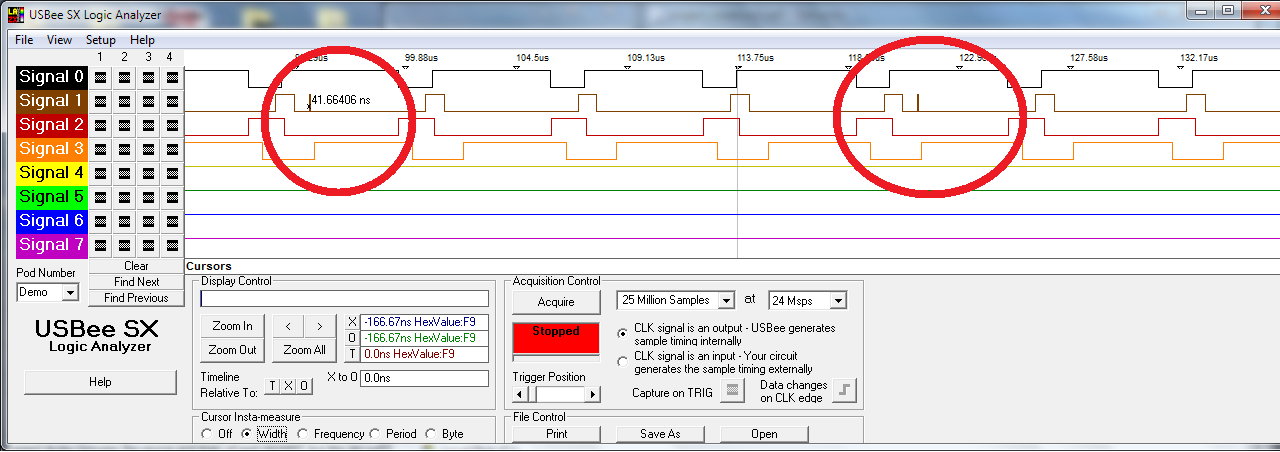
\includegraphics[scale=0.33]{img/switch_glitch.png}

Noticing that the amp could become unstable at times with the DC blocking capacitor in the feedback loop, I rewired the analog front end to eliminate the need for this capacitor.  Instead of powering the input op-amp and comparator off of 5V as I had been doing, I now power them off of the full input voltage.  The input is limited to 30V by the gate driver, so no specs should be exceeded in doing this.  Additionally, the comparator output is open-collector, so logic level interfacing between the gate driver and comparator is done inherently and no special attention is needed to accomplish it.  A second op-amp channel is still used to create an internal low-current \(\frac{V_{CC}}{2}\) rail, but this rail now operates at half the supply voltage instead of 2.5V.

A new problem was introduced, though.  If the requested output is greater than what the MOSFETs can supply for any period of time, the amplifier can stop oscillating.  Luckily, the failure mode happens such that one half-bridge stops conducting completely, so a speaker-destroying DC current does not appear across the speaker.  This issue will have to be dealt with prior to ordering amplifier PCBs.  One potential correctional measure is to include an additional triangle-wave based modulator.
\end{nbentry}

\end{document}
